% This is the template for submission of abstracts to NetSci 2024 in Québec, Canada.
% It is modified from NetSci2017, which was inspired by that of NetSci2016 and that of STATPHSY25.
% The editor of the booklet reserves the right to modify your submission.

% To process this file run LaTeX2e

% ******** DO NOT EDIT ****************
\documentclass[10pt]{article}
% \usepackage{mathptmx}
\usepackage[letterpaper,margin=20mm]{geometry}
\usepackage{graphicx}
\usepackage{lmodern}
\renewcommand{\familydefault}{\sfdefault}
\pagestyle{empty}
\setlength{\parskip}{0.25\baselineskip}
\renewcommand{\title}[1]{{\noindent\large\bfseries#1\medskip\\}}
\renewcommand{\author}[2]{{\noindent #1 \medskip\\ \noindent \small #2 \medskip\\}}
% *************************************

\begin{document}

% ********** USER DEFINED *************


% Enter title here
\title{A Regional Spatial Graph Convolutional Neural Network (RSGCN) for Spatially Embedded Network Modeling}
\author{
    % Enter author(s) here
    Xudong Fan\textsuperscript{1}
    and
    Jürgen Hackl,\textsuperscript{1}
}
{
    % Enter affiliation(s) here
    1. Princeton University, Princeton, NJ, USA\\
}



% Enter abstract here. Please keep everything within one page.
Network modeling provides a structured and abstract representation of real-world infrastructure systems, such as road networks and power networks. It has also enabled various analyses and optimizations for infrastructure systems management. In order to accurately model critical infrastructure networks and generate realistic network data, this study proposed a regional spatial graph convolutional network (RSGCN) for network connection prediction. Unlike traditional graph theory-based models which assume the graphs are independent of the space, the proposed method assumes the critical infrastructure are spatially embedded networks. The spatial information of the infrastructure has been considered in the network modeling process and thereby achieved a higher model accuracy. To test and evaluate the performance of the proposed model, three graph datasets were used for training and validating purposes, including a synthetic graph dataset, a real-world road network, and a real-world power network. The modeling results of RSGCN were then compared to those of two other geometric deep learning models, GraphSAGE and Spatial Graph Convolutional Network (SGCN). It was found that the proposed RSGCN outperformed the weakest model by 6.65\%, 37\%, and 59\%, respectively, regarding the F1 score in the three datasets. The proposed model also predicted a more accurate edge length distribution, node degree distribution, and number of component distribution, compared to the other models. The proposed method is the first variant of graph convolutional networks (GCNs) that can take regional spatial information into account and can be deployed for modeling critical infrastructure networks.


\begin{figure}[!h]
    \centering
    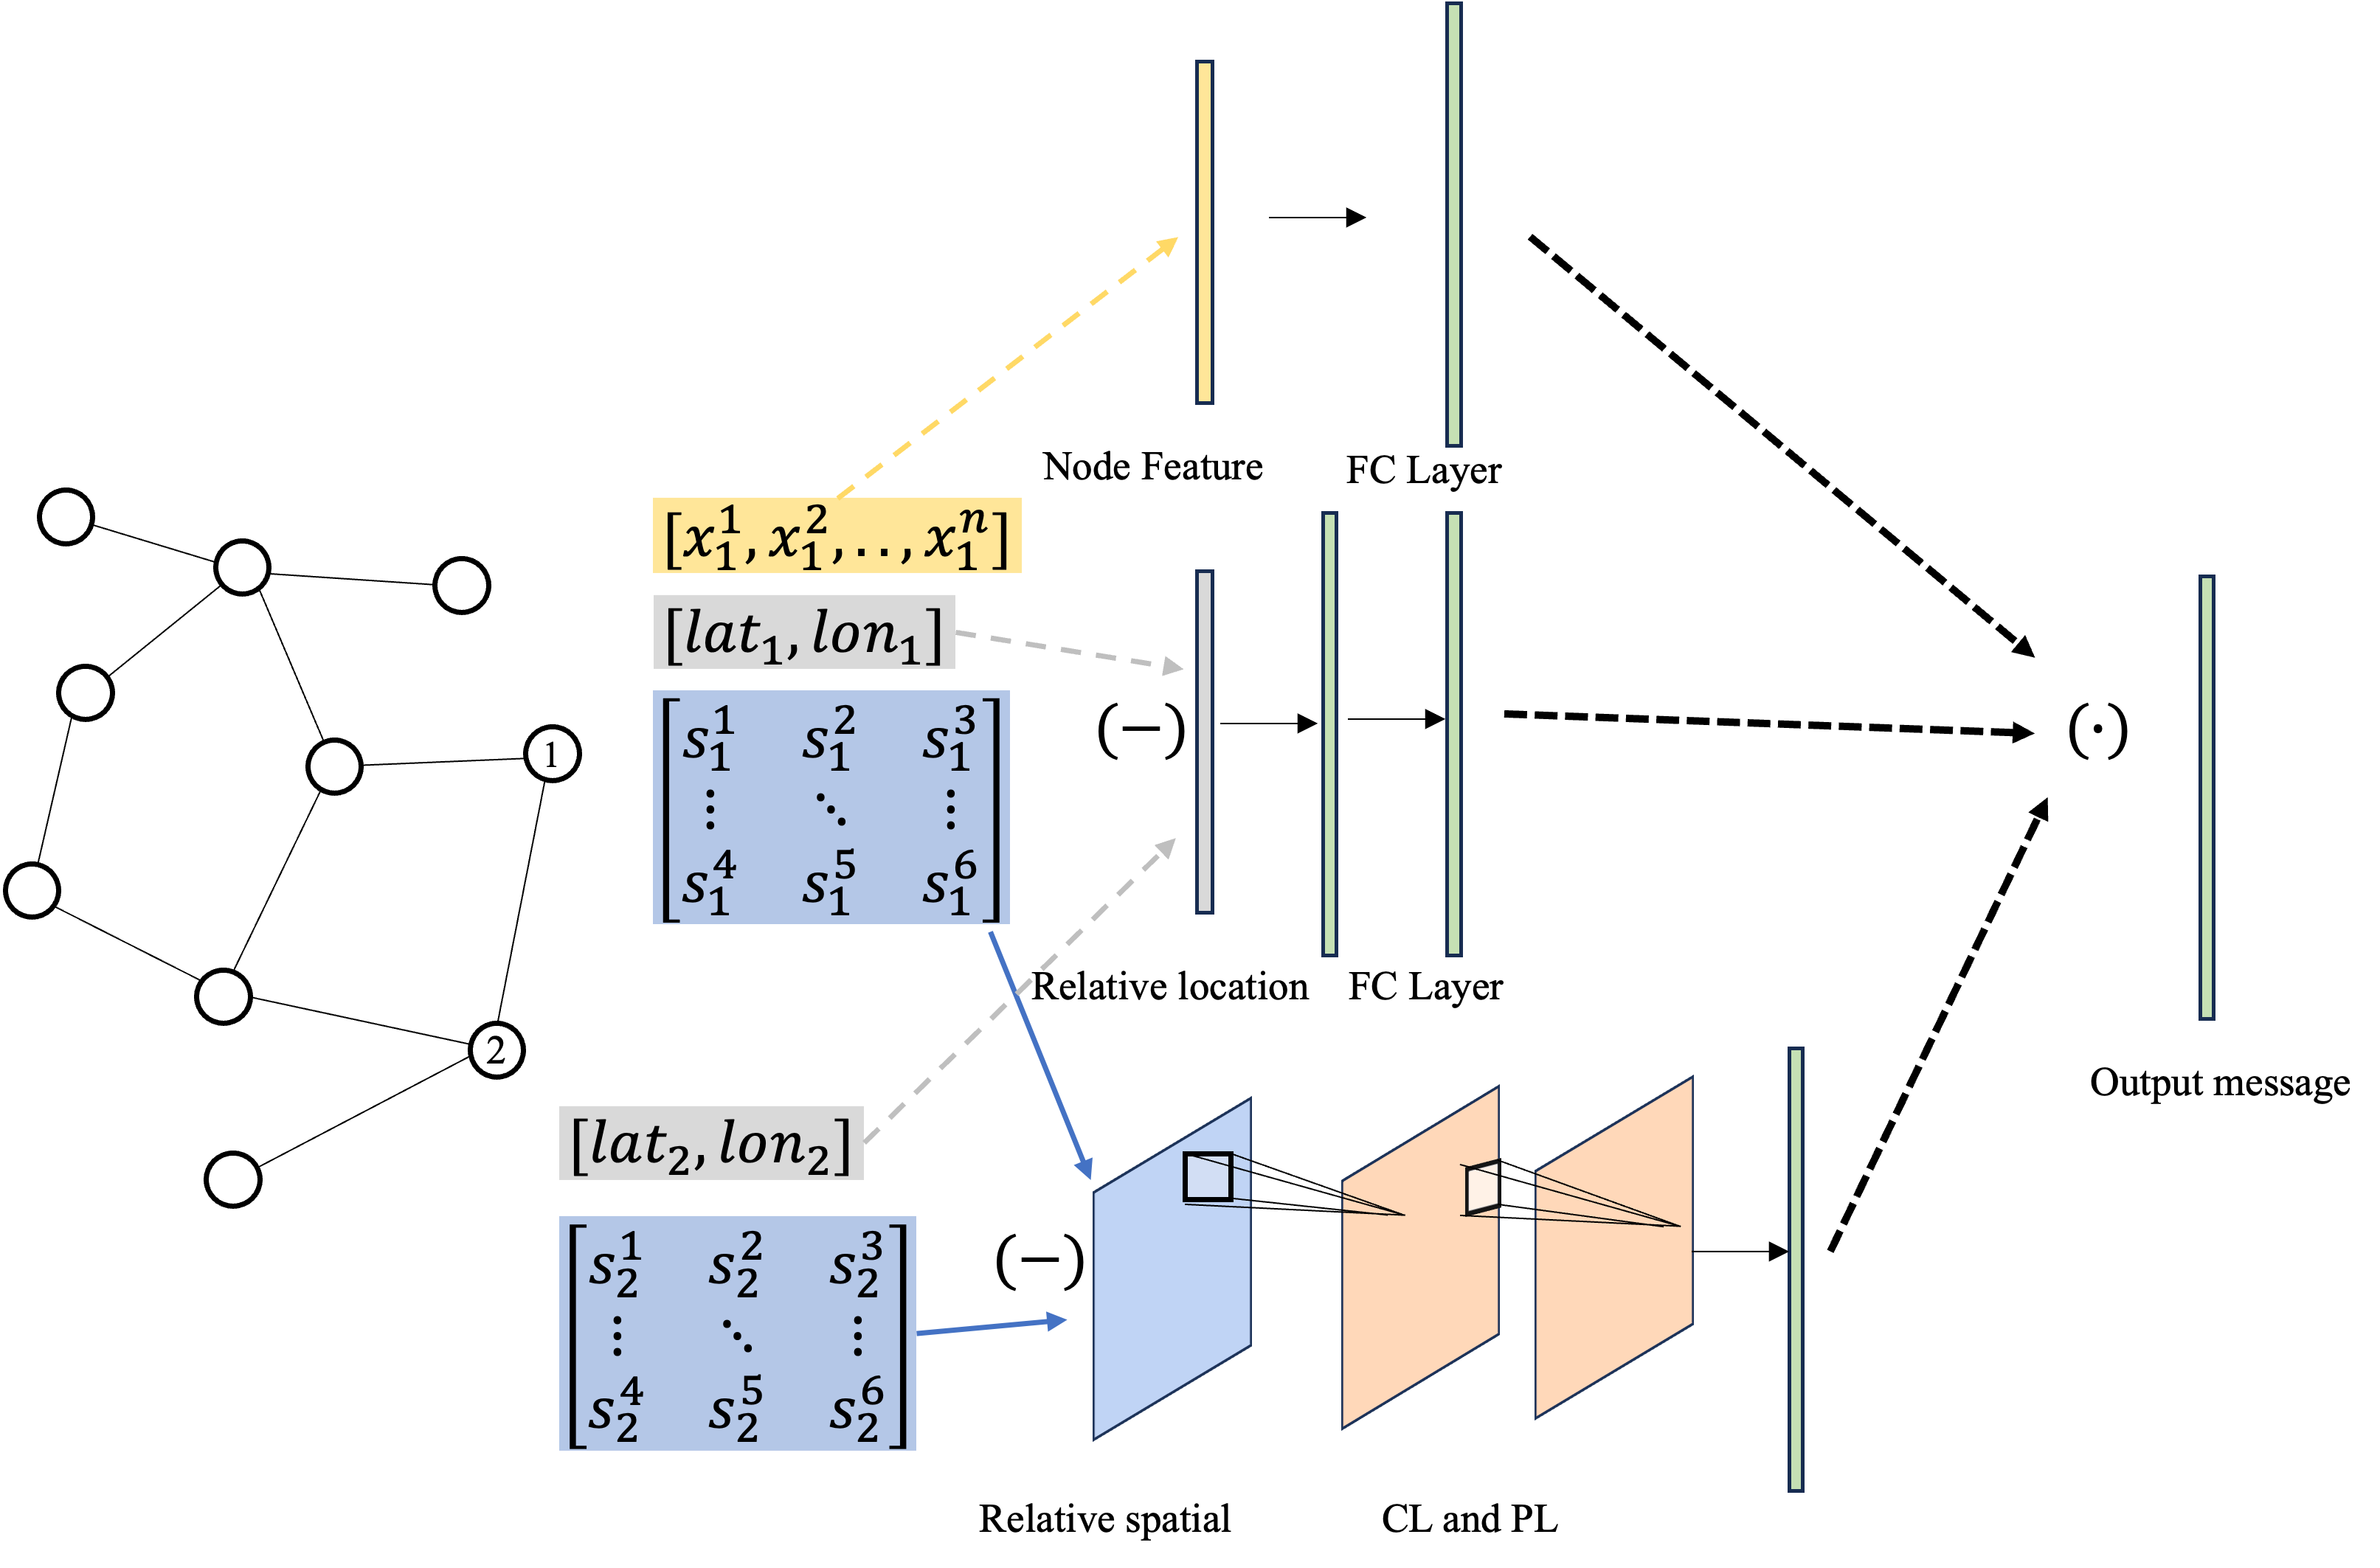
\includegraphics[width=0.6\textwidth]{RSGCN.png}
    \caption{\textbf{The Proposed RSGCN Architecture}}
\end{figure}


% *************************************
\end{document}